\documentclass[border=10pt]{standalone}
\usepackage{tikz}

\begin{document}

\begin{tikzpicture}
    % Text box styling
    \draw[fill=yellow!30, draw=black, rounded corners] (0,0) rectangle (6,4);
    
    % Text content
    \node at (1,2) {\footnotesize As a restaurant manager, you want to determine the optimal pricing strategy for a popular menu item. The demand function for this item is nonlinear and given by $q = 1000 - 10p^2$, where $q$ is the quantity demanded and $p$ is the price in dollars. The cost to produce each unit is \$5. What price should you set to maximize profit, and what is the maximum profit?};
\end{tikzpicture}

\end{document}